\subsection{中心極限定理の確認}

\subsubsection{一様乱数の場合}\label{subsubsec:cl-uniform}
一様乱数に従う乱数を生成し、その和を取る操作を繰り返すことで中心極限定理を確認する。
元々の一様分布が図\ref{fig:cl-uniform-original}であり、そのQQプロットが図\ref{fig:cl-uniform-original-qqpl}である。
この分布に一様乱数を加算した場合の分布が図\ref{fig:cl-uniform-added}であり、そのQQプロットが図\ref{fig:cl-uniform-added-qqpl}である。
図\ref{fig:cl-uniform-added-qqpl}をみると、加算した場合も正規分布に従っていることがわかり中心極限定理が成り立っていることがわかる。
標準正規分布のQQプロットである、図\ref{fig:cl-uniform-original-qqpl}と比較すると、一様乱数の場合は-4や4付近での値が多く、端の部分で図\ref{fig:cl-uniform-original-qqpl}にあるように引っ張られたような形になっている。
\begin{figure}
	\centering
	\begin{subfigure}{0.48\linewidth}
		\centering
		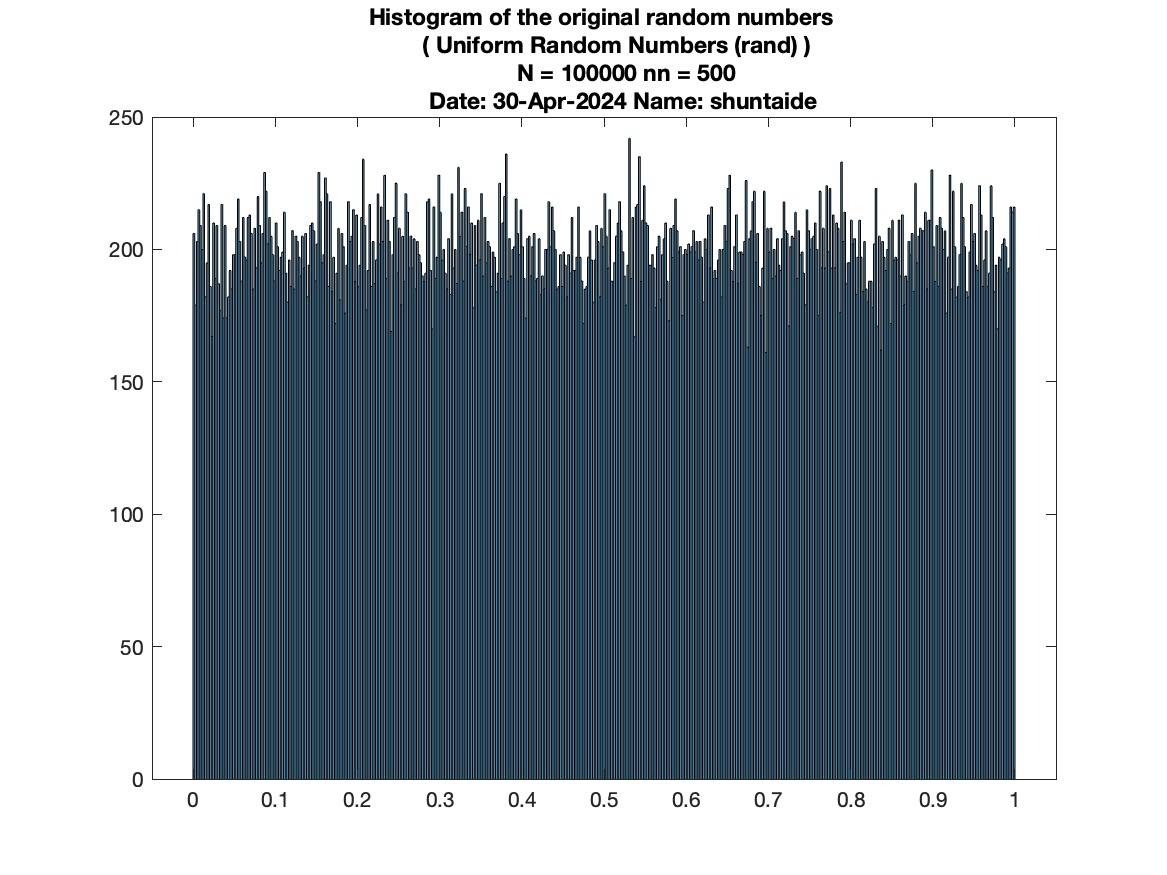
\includegraphics[width=0.8\textwidth]{src/figures/cl-uniform/cl_original_rand_hist_N=100000_nn=500.jpg}
		\subcaption{元々の分布}\label{fig:cl-uniform-original}
	\end{subfigure}
	\begin{subfigure}{0.48\linewidth}
		\centering
		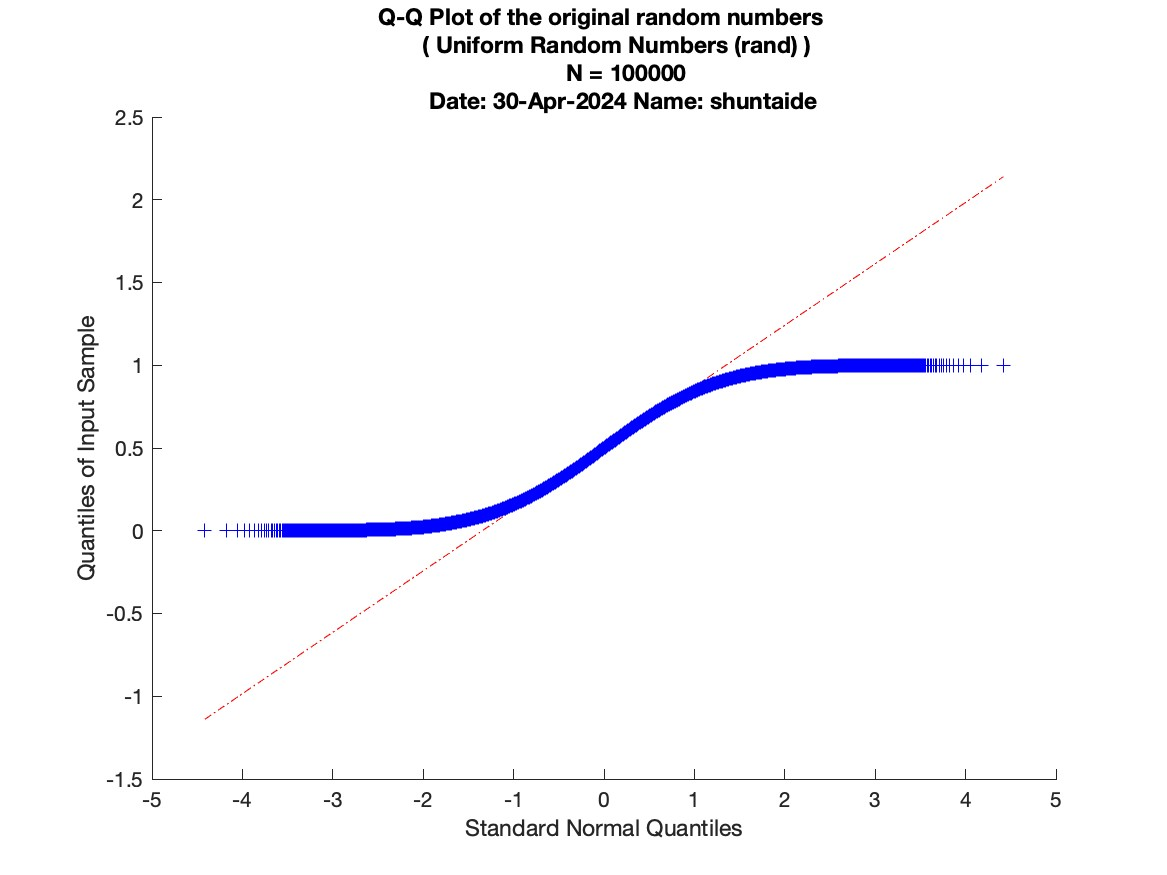
\includegraphics[width=0.8\textwidth]{src/figures/cl-uniform/cl_original_rand_qqpl_N=100000.jpg}
		\subcaption{元々の分布のQQプロット}\label{fig:cl-uniform-original-qqpl}
	\end{subfigure}
	\begin{subfigure}{0.48\linewidth}
		\centering
		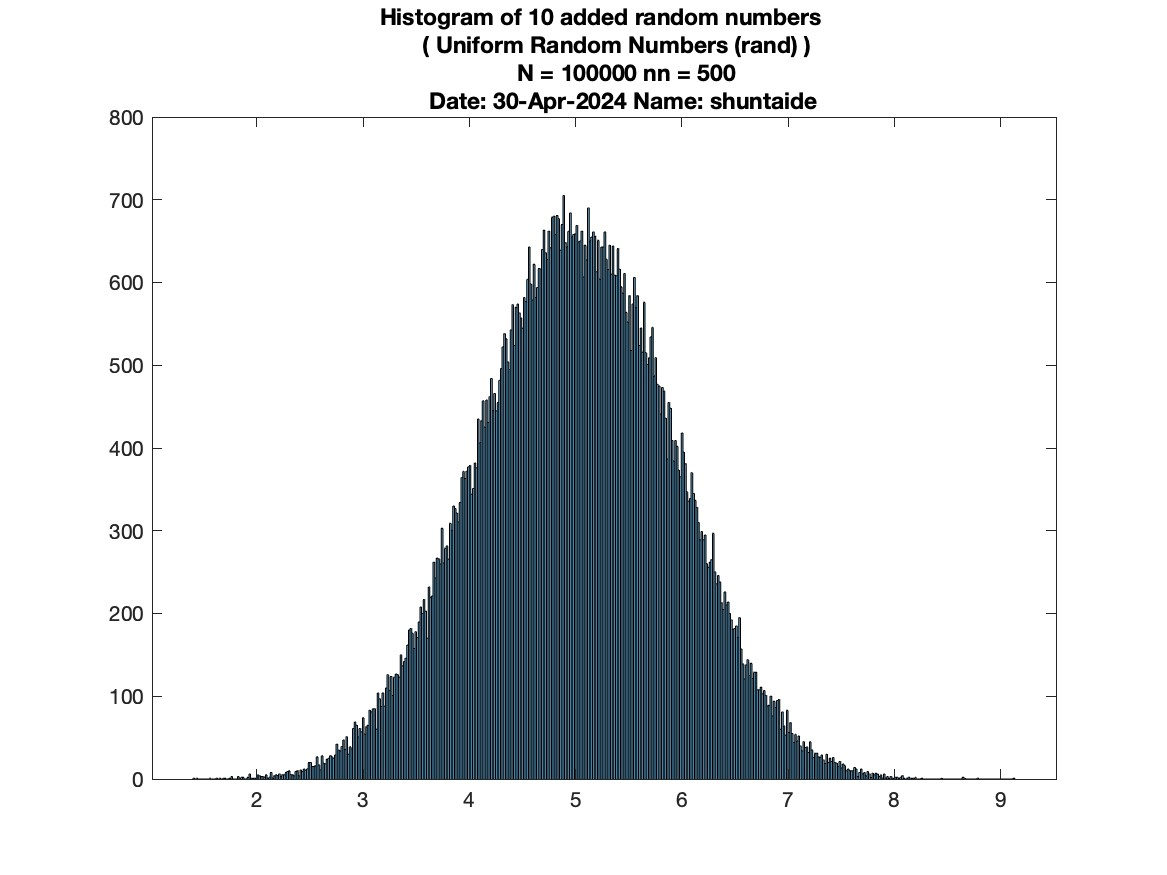
\includegraphics[width=0.8\textwidth]{src/figures/cl-uniform/cl_added_rand_hist_N=100000_nn=500.jpg}
		\subcaption{加算した分布}\label{fig:cl-uniform-added}
	\end{subfigure}
	\begin{subfigure}{0.48\linewidth}
		\centering
		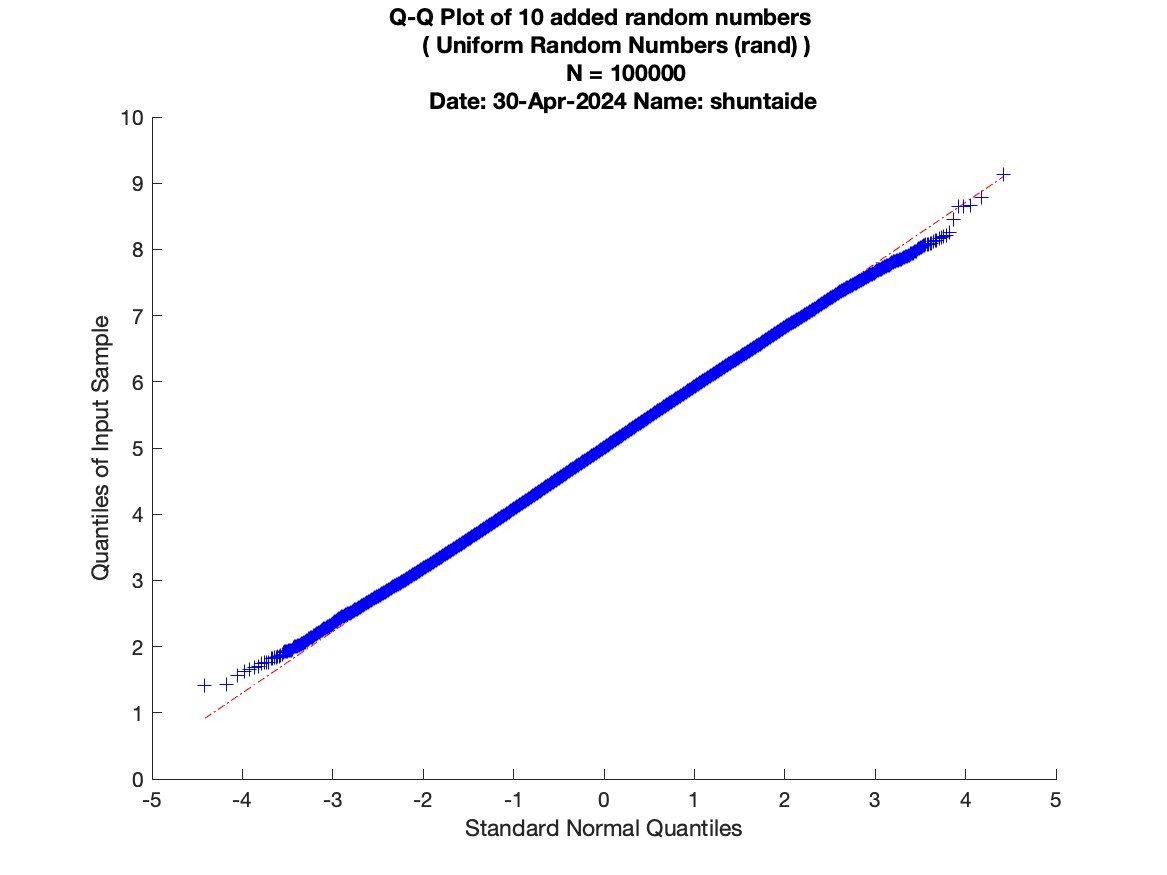
\includegraphics[width=0.8\textwidth]{src/figures/cl-uniform/cl_added_rand_qqpl_N=100000.jpg}
		\subcaption{加算した分布のQQプロット}\label{fig:cl-uniform-added-qqpl}
	\end{subfigure}
	\caption{一様乱数による生成結果}\label{fig:cl-uniform-random}
\end{figure}


\subsubsection{標準正規乱数の場合}\label{subsubsec:cl-standard-normal}
標準正規分布にしたがう乱数を生成し、その和を取る操作を繰り返すことで中心極限定理を確認する。
元々の標準正規分布が図\ref{fig:cl-standard-normal-original}であり、そのQQプロットが図\ref{fig:cl-standard-normal-original-qqpl}である。
この分布に標準正規乱数を加算した場合の分布が図\ref{fi:cl-standard-normal-added}であり、そのQQプロットが図\ref{fig:cl-standard-normal-added-qqpl}である。
図\ref{fig:cl-standard-normal-added-qqpl}をみると、加算した場合も正規分布に従っていることがわかり中心極限定理が成り立っていることがわかる。
\begin{figure}
	\centering
	\begin{subfigure}{0.48\linewidth}
		\centering
		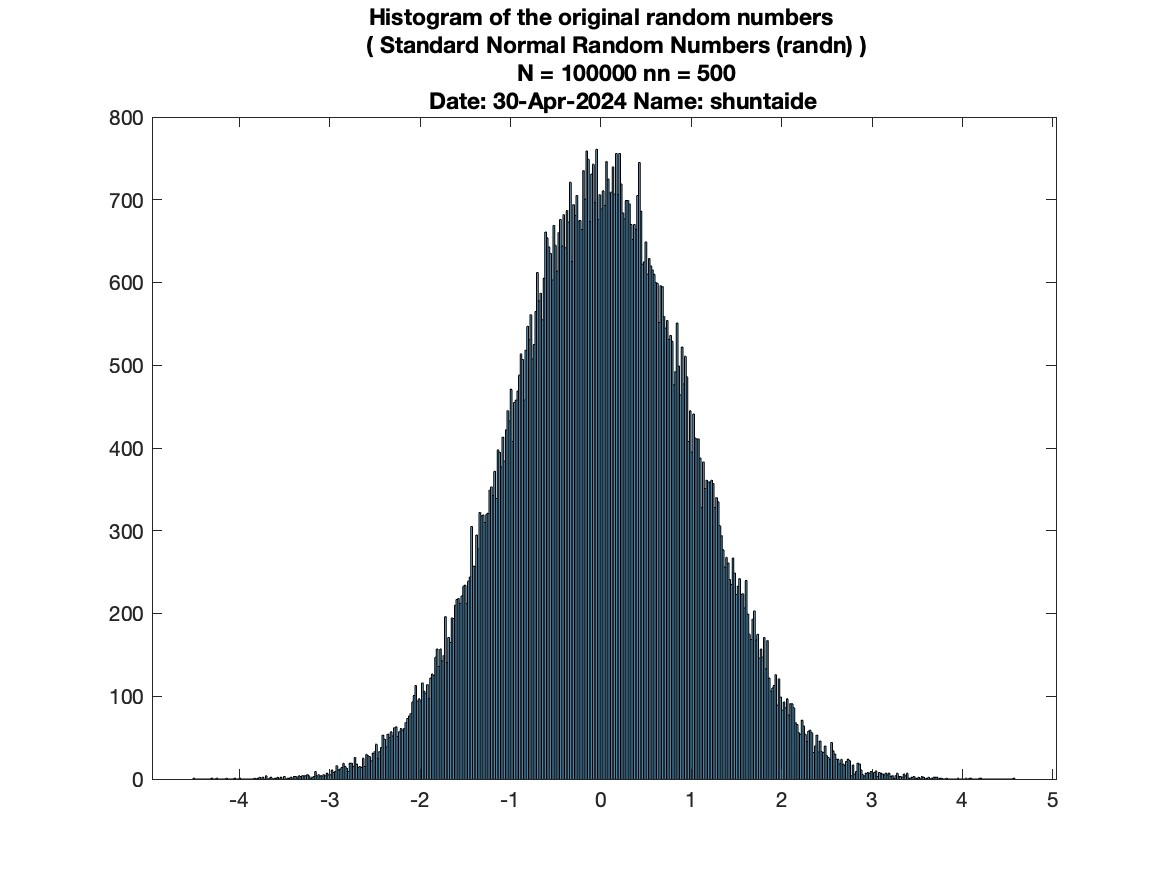
\includegraphics[width=0.8\textwidth]{src/figures/cl-standard-normal/cl_original_randn_hist_N=100000_nn=500.jpg}
		\subcaption{元々の分布}\label{fig:cl-standard-normal-original}
	\end{subfigure}
	\begin{subfigure}{0.48\linewidth}
		\centering
		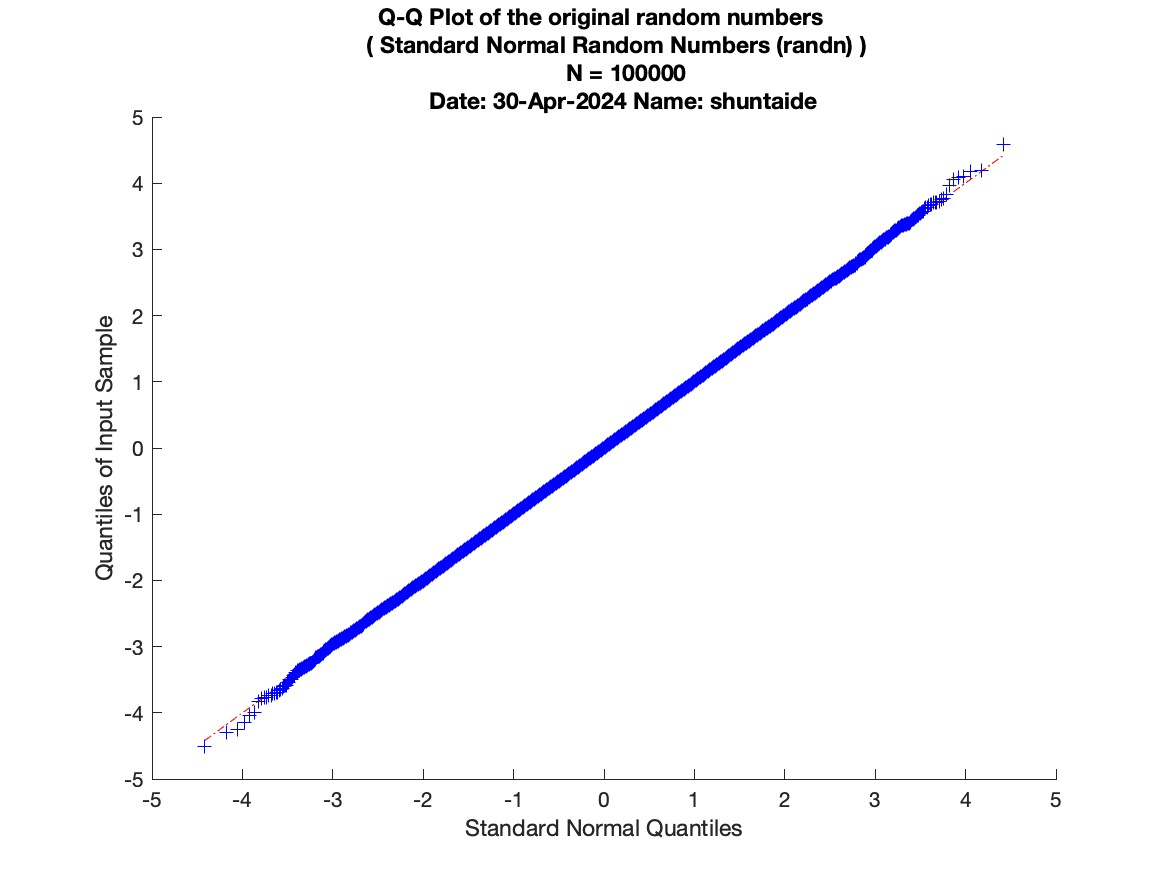
\includegraphics[width=0.8\textwidth]{src/figures/cl-standard-normal/cl_original_randn_qqpl_N=100000.jpg}
		\subcaption{元々の分布のQQプロット}\label{fig:cl-standard-normal-original-qqpl}
	\end{subfigure}
	\begin{subfigure}{0.48\linewidth}
		\centering
		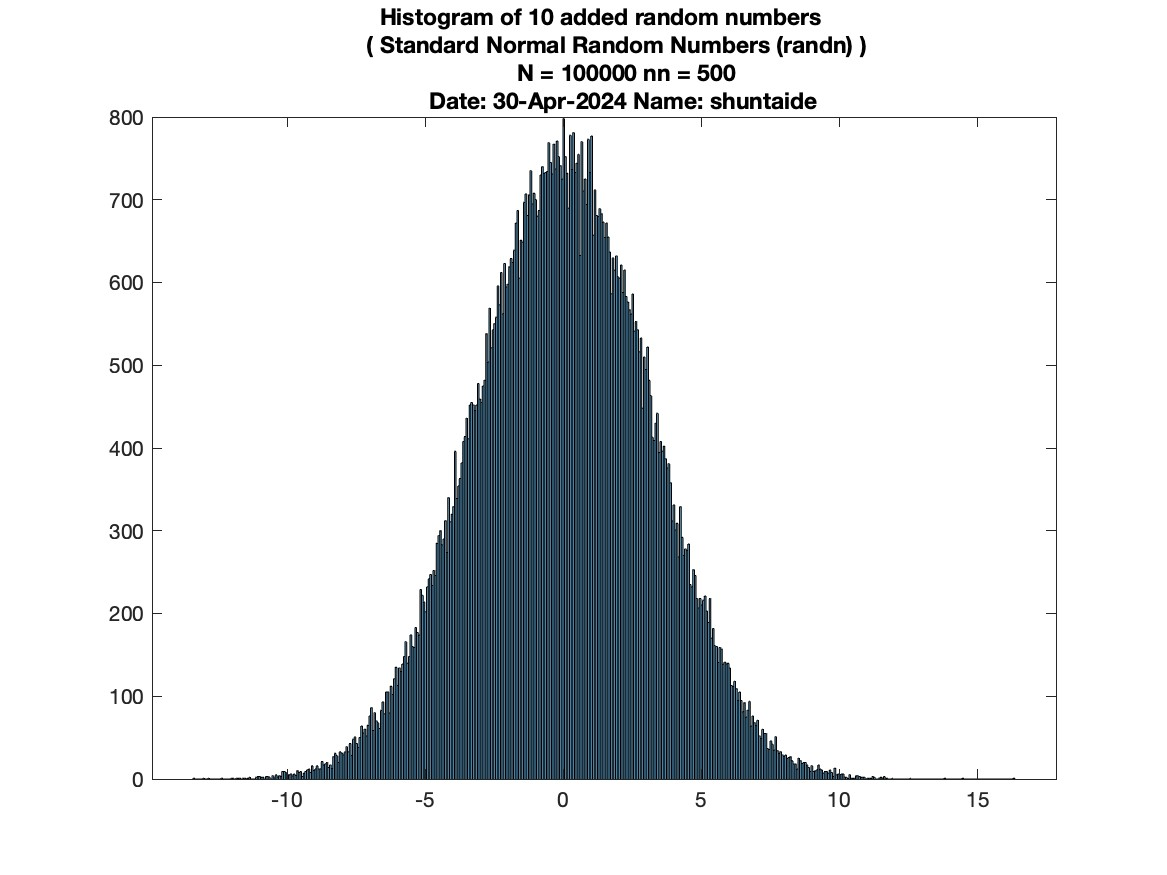
\includegraphics[width=0.8\textwidth]{src/figures/cl-standard-normal/cl_added_randn_hist_N=100000_nn=500.jpg}
		\subcaption{加算した場合の分布}\label{fi:cl-standard-normal-added}
	\end{subfigure}
	\begin{subfigure}{0.48\linewidth}
		\centering
		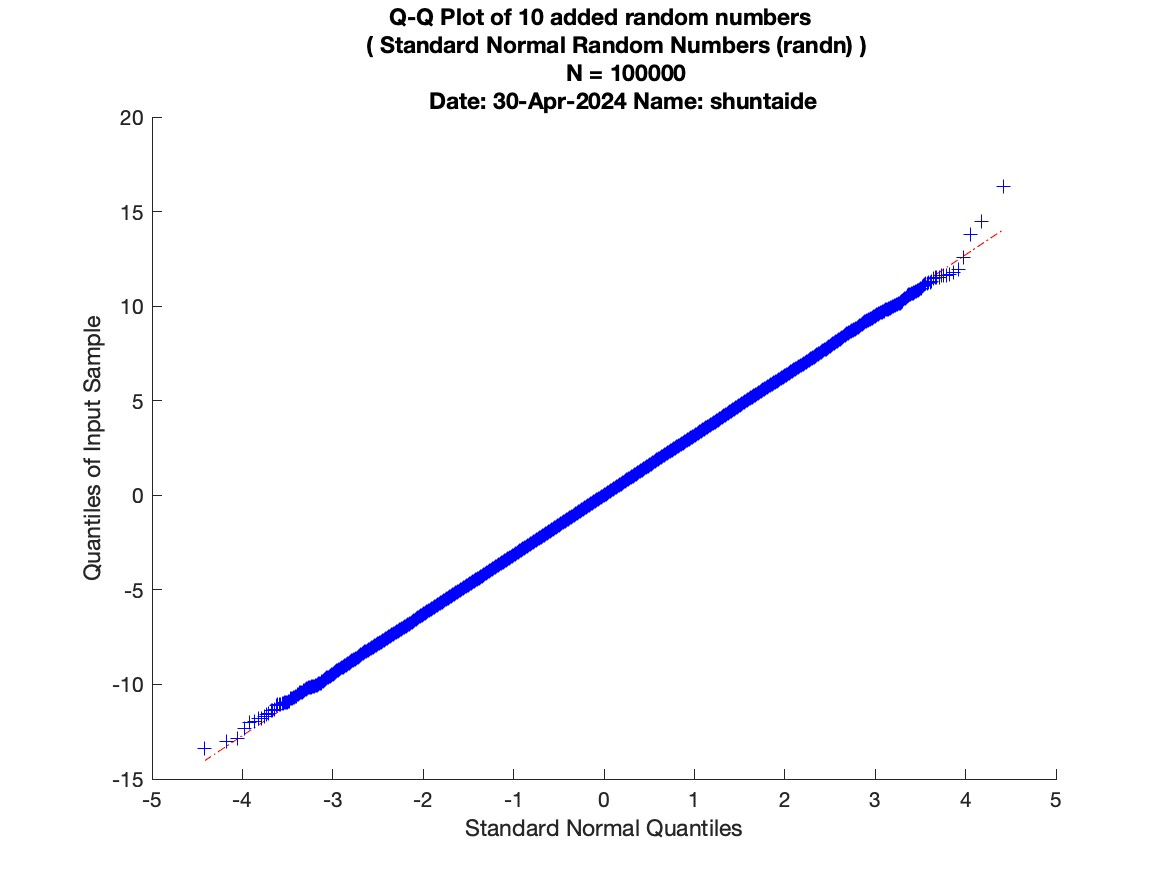
\includegraphics[width=0.8\textwidth]{src/figures/cl-standard-normal/cl_added_randn_qqpl_N=100000.jpg}
		\subcaption{加算した場合のQQプロット}\label{fig:cl-standard-normal-added-qqpl}
	\end{subfigure}
	\caption{標準正規乱数による生成結果}\label{fig:cl-standard-normal-random}
\end{figure}


\subsubsection{指数分布の場合}\label{subsubsec:cl-exp}
指数分布に従う乱数を生成し、その和を取る操作を繰り返すことで中心極限定理を確認する。
元々の指数分布が図\ref{fig:cl-exp-original}であり、そのQQプロットが図\ref{fig:cl-exp-original-qqpl}である。
この分布に指数分布に従う乱数を加算した場合の分布が図\ref{fig:cl-exp-added}であり、そのQQプロットが図\ref{fig:cl-exp-added-qqpl}である。
図\ref{fig:cl-exp-added-qqpl}をみると、加算した場合元の指数分布よりは正規分布に近い形であるが、正規分布より小さい値が多く偏っていることがわかる。
一様分布の場合である\ref{subsubsec:cl-standard-normal}に比べて、形が正規分布に近くなっていない。
\begin{figure}
	\centering
	\begin{subfigure}{0.48\linewidth}
		\centering
		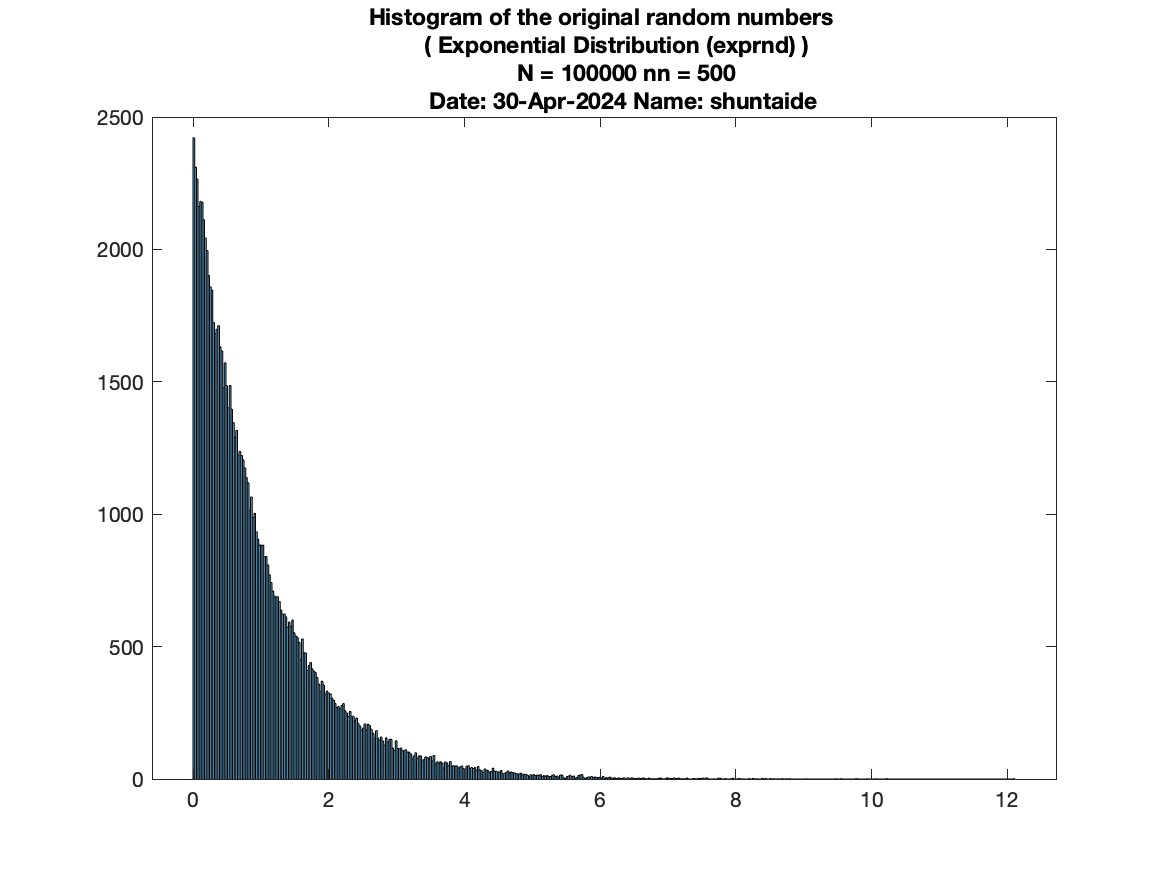
\includegraphics[width=0.8\textwidth]{src/figures/cl-exp/cl_original_exprnd_hist_N=100000_nn=500.jpg}
		\subcaption{元々の分布}\label{fig:cl-exp-original}
	\end{subfigure}
	\begin{subfigure}{0.48\linewidth}
		\centering
		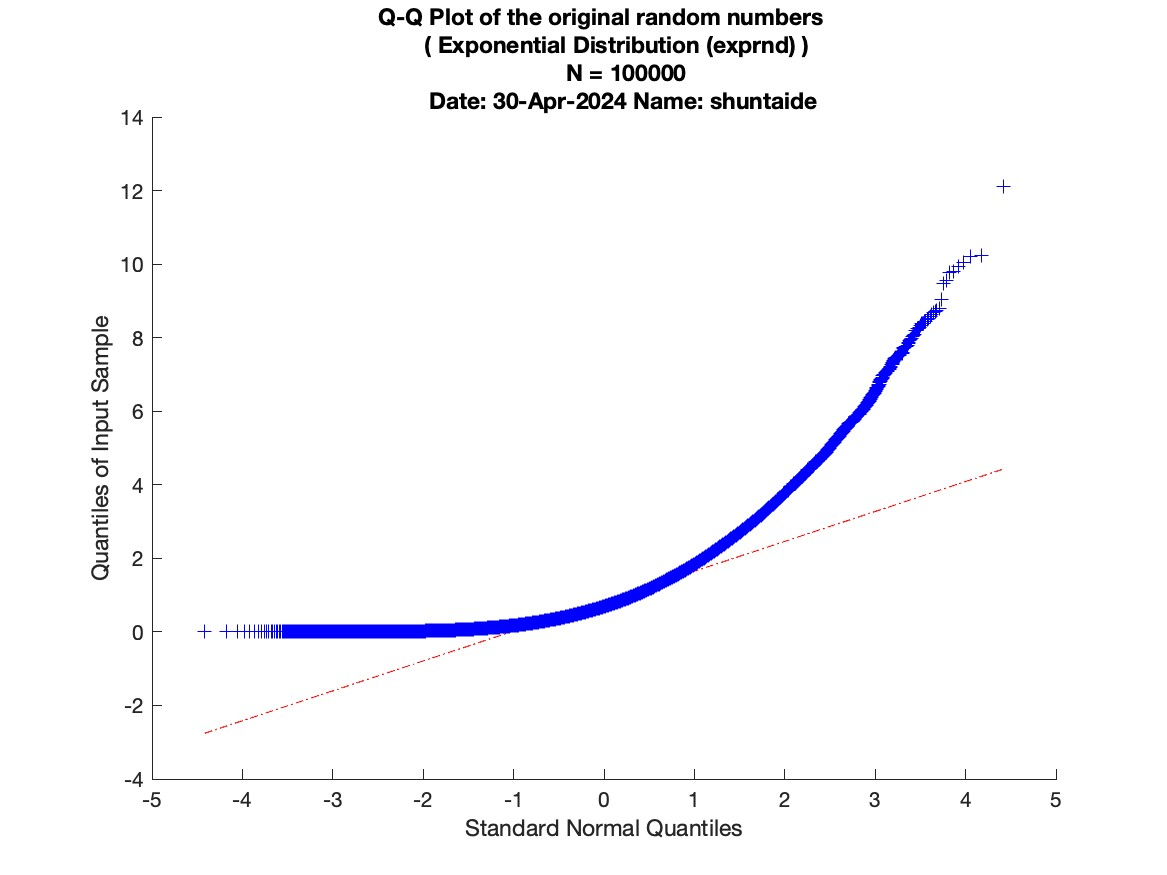
\includegraphics[width=0.8\textwidth]{src/figures/cl-exp/cl_original_exprnd_qqpl_N=100000.jpg}
		\subcaption{QQプロット}\label{fig:cl-exp-original-qqpl}
	\end{subfigure}
	\begin{subfigure}{0.48\linewidth}
		\centering
		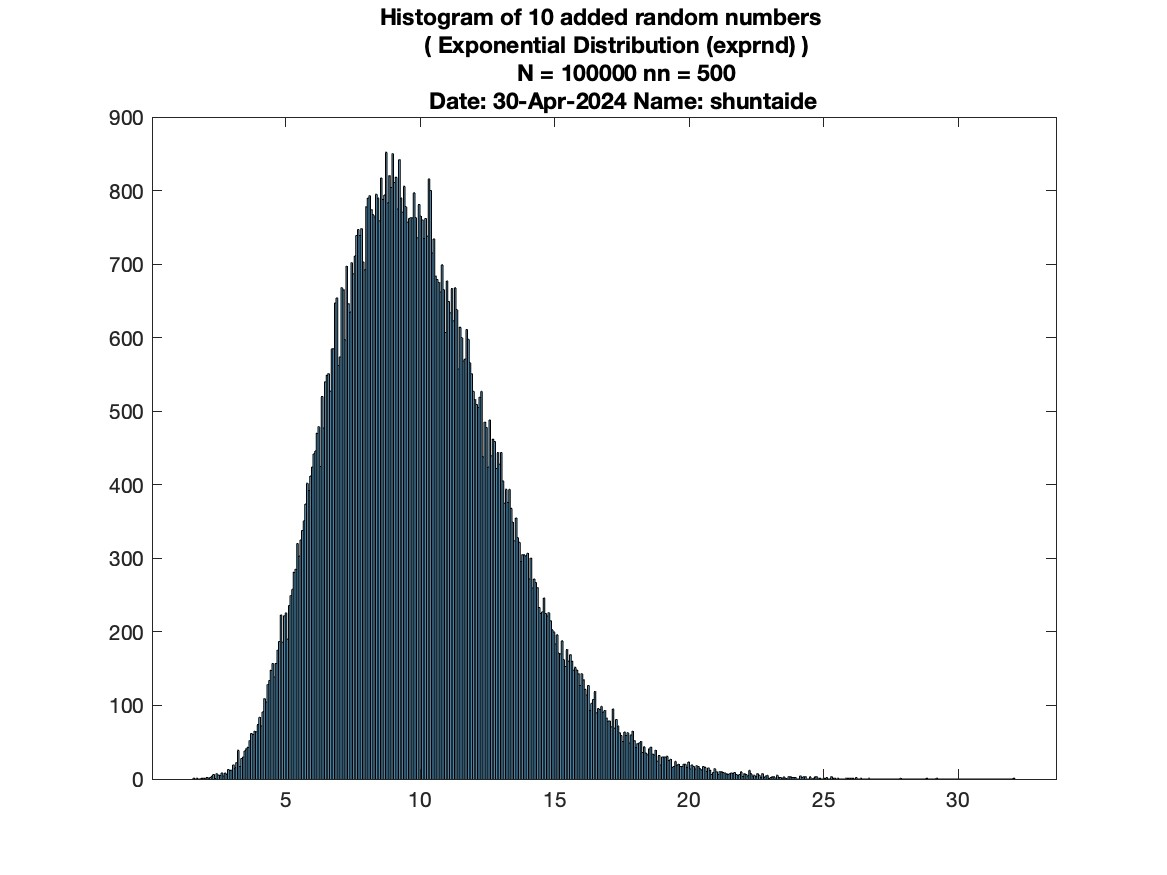
\includegraphics[width=0.8\textwidth]{src/figures/cl-exp/cl_added_exprnd_hist_N=100000_nn=500.jpg}
		\subcaption{加算後の分布}\label{fig:cl-exp-added}
	\end{subfigure}
	\begin{subfigure}{0.48\linewidth}
		\centering
		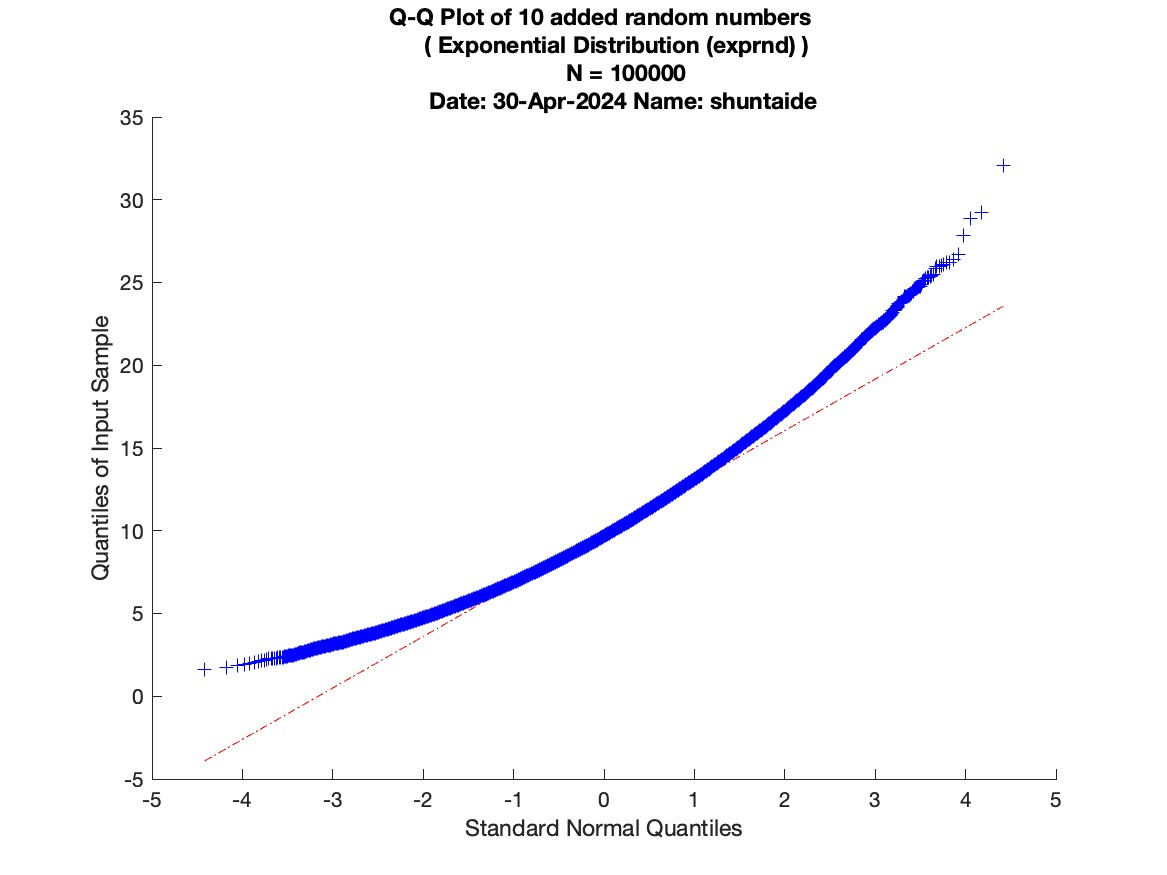
\includegraphics[width=0.8\textwidth]{src/figures/cl-exp/cl_added_exprnd_qqpl_N=100000.jpg}
		\subcaption{加算後のQQプロット}\label{fig:cl-exp-added-qqpl}
	\end{subfigure}
	\caption{指数分布による生成結果}\label{fig:cl-exp-random}
\end{figure}


\subsubsection{ガンマ分布の場合}\label{subsubsec:cl-gamma}
ガンマ分布に従う乱数を生成し、その和を取る操作を繰り返すことで中心極限定理を確認する。
元々のガンマ分布が図\ref{fig:cl-gamma-original}であり、そのQQプロットが図\ref{fig:cl-gamma-original-qqpl}である。
この分布にガンマ分布に従う乱数を加算した場合の分布が図\ref{fig:cl-gamma-added}であり、そのQQプロットが図\ref{fig:cl-gamma-added-qqpl}である。
図\ref{fig:cl-gamma-added-qqpl}をみると、加算した場合元のガンマ分布よりは正規分布に近い形であるが、正規分布より小さい値が多く偏っていることがわかる。
一様分布の場合である\ref{subsubsec:cl-standard-normal}に比べて、形が正規分布に近くなっていないが、
指数分布の場合である\ref{subsubsec:cl-exp}に比べるとほぼ形が同じである。
\begin{figure}
	\centering
	\begin{subfigure}{0.48\linewidth}
		\centering
		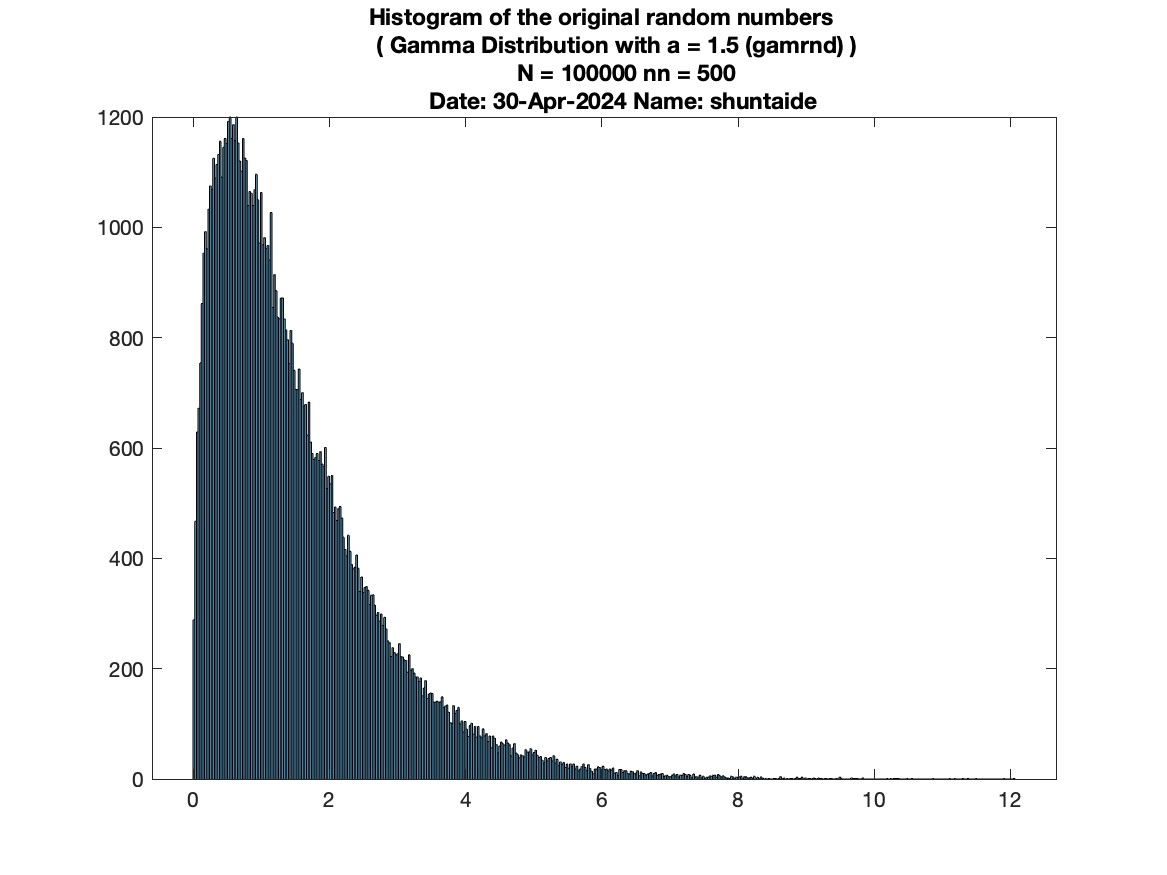
\includegraphics[width=0.8\textwidth]{src/figures/cl-gamma/cl_original_gamrnd_hist_N=100000_nn=500.jpg}
		\subcaption{元々の分布}\label{fig:cl-gamma-original}
	\end{subfigure}
	\begin{subfigure}{0.48\linewidth}
		\centering
		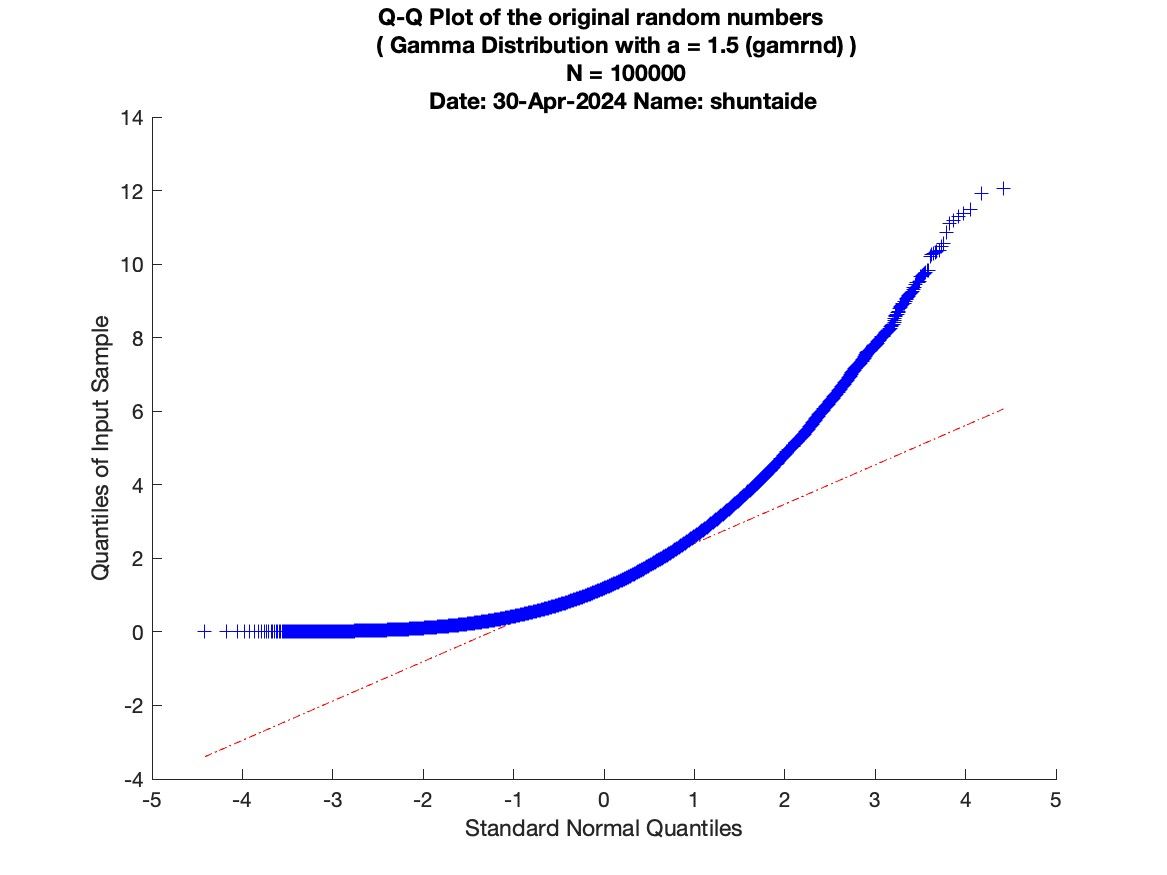
\includegraphics[width=0.8\textwidth]{src/figures/cl-gamma/cl_original_gamrnd_qqpl_N=100000.jpg}
		\subcaption{元々の分布のQQプロット}\label{fig:cl-gamma-original-qqpl}
	\end{subfigure}
	\begin{subfigure}{0.48\linewidth}
		\centering
		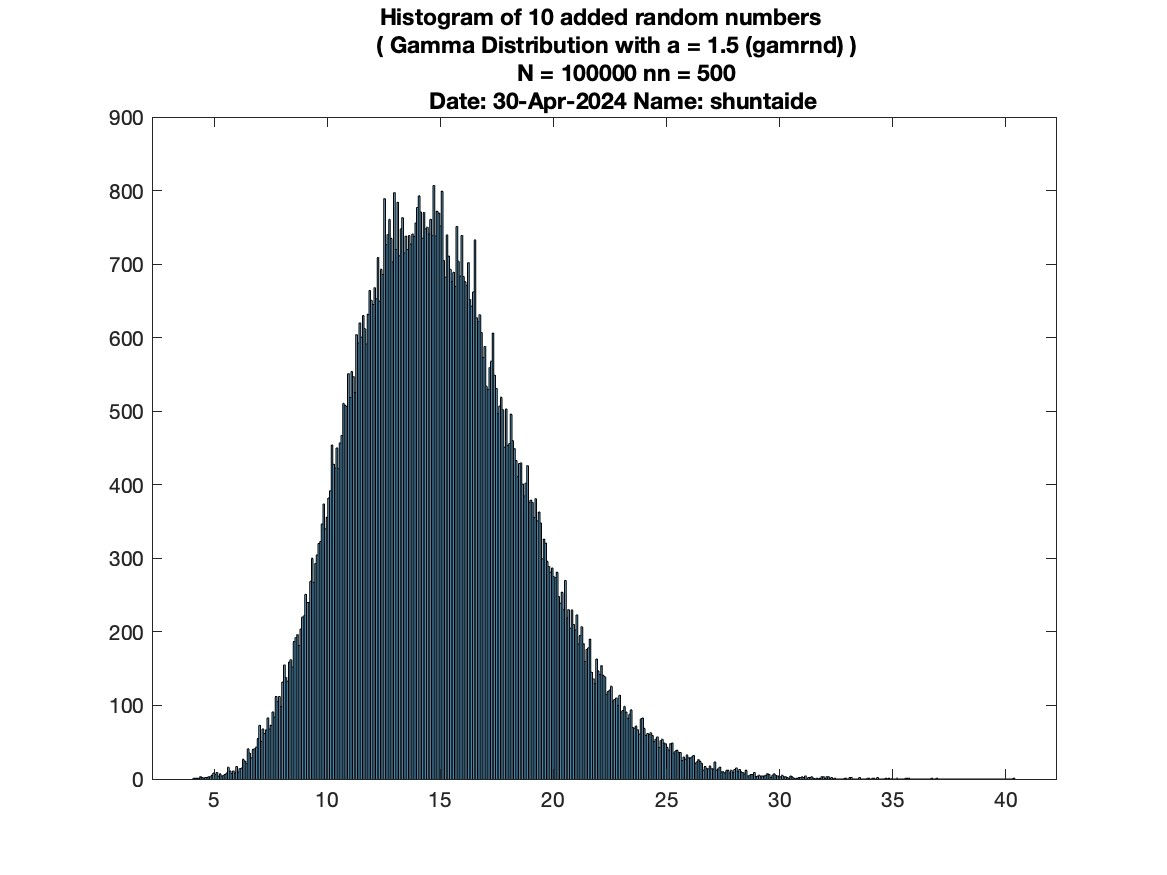
\includegraphics[width=0.8\textwidth]{src/figures/cl-gamma/cl_added_gamrnd_hist_N=100000_nn=500.jpg}
		\subcaption{加算した分布}\label{fig:cl-gamma-added}
	\end{subfigure}
	\begin{subfigure}{0.48\linewidth}
		\centering
		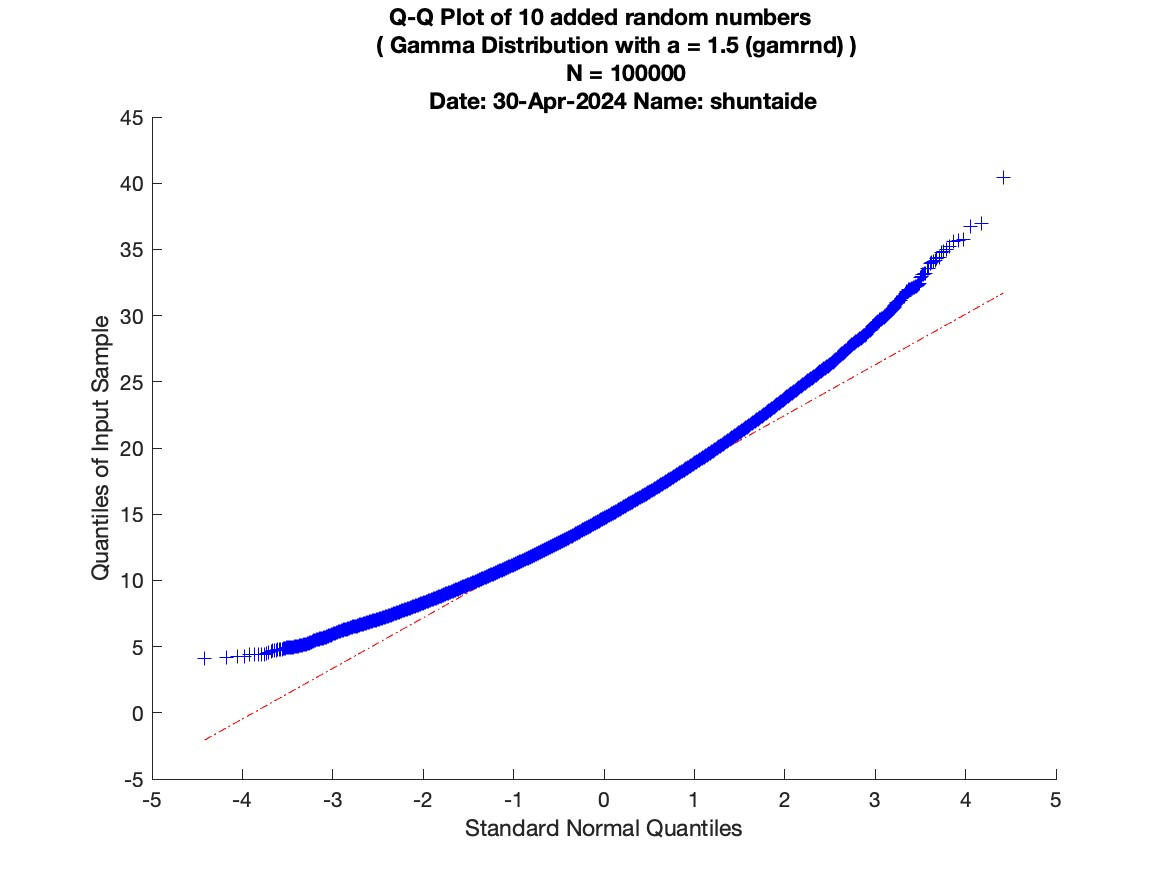
\includegraphics[width=0.8\textwidth]{src/figures/cl-gamma/cl_added_gamrnd_qqpl_N=100000.jpg}
		\subcaption{加算した分布のQQプロット}\label{fig:cl-gamma-added-qqpl}
	\end{subfigure}
	\caption{ガンマ分布による生成結果}\label{fig:cl-gamma-random}
\end{figure}


\subsubsection{ポアソン分布の場合}\label{subsubsec:cl-poisson}
ポアソン分布に従う乱数を生成し、その和を取る操作を繰り返すことで中心極限定理を確認する。
元々のポアソン分布が図\ref{fig:cl-poisson-original}であり、そのQQプロットが図\ref{fig:cl-poisson-original-qqpl}である。
この分布にポアソン分布に従う乱数を加算した場合の分布が図\ref{fig:cl-poisson-added}であり、そのQQプロットが図\ref{fig:cl-poisson-added-qqpl}である。
図\ref{fig:cl-poisson-added-qqpl}をみると、加算した場合元のポアソン分布よりは正規分布に近い形であるが、正規分布より小さい値が多く偏っていることがわかる。
一様分布の場合である\ref{subsubsec:cl-standard-normal}に比べて、形が正規分布に近くなっていないが、
指数分布の場合である\ref{subsubsec:cl-exp}やガンマ分布である\ref{subsubsec:cl-gamma}に比べるとほぼ形が同じである。
\begin{figure}
	\centering
	\begin{subfigure}{0.48\linewidth}
		\centering
		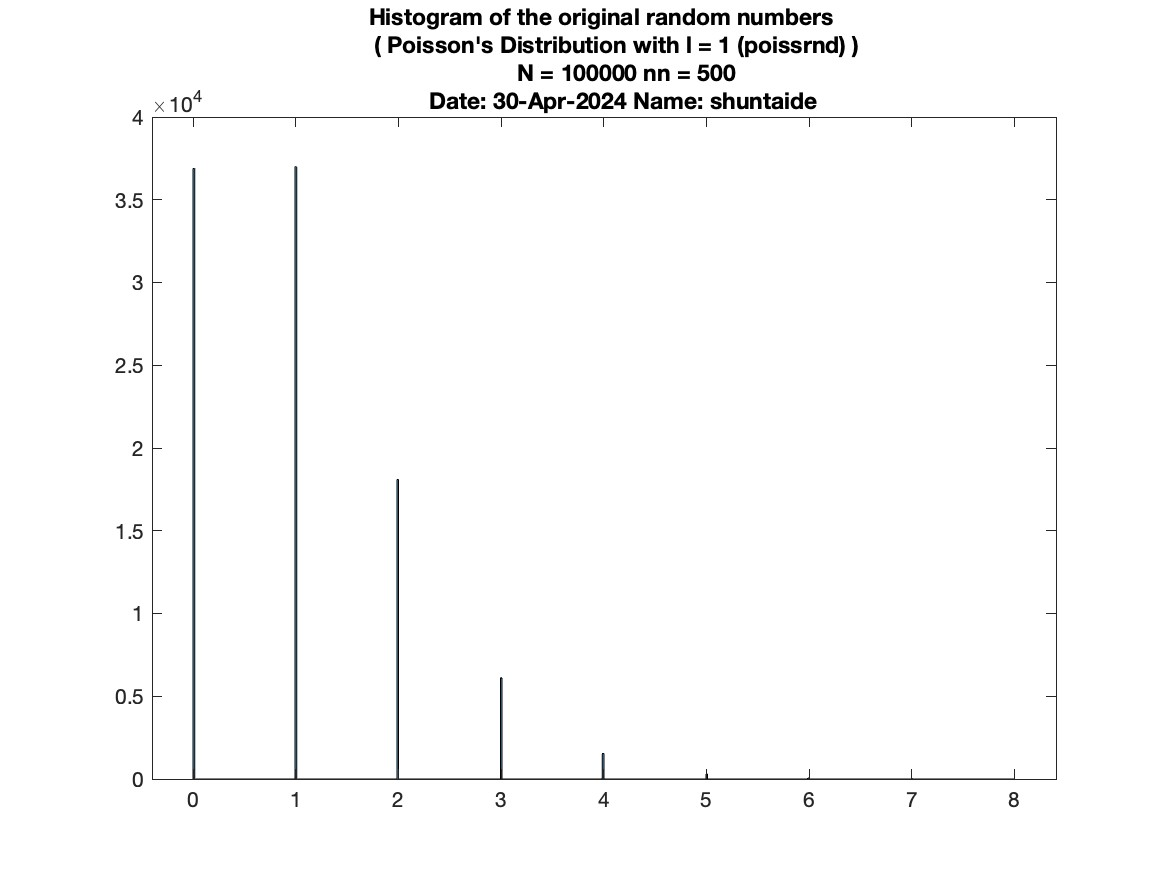
\includegraphics[width=0.8\textwidth]{src/figures/cl-poisson/cl_original_poissrnd_hist_N=100000_nn=500.jpg}
		\subcaption{元々の分布}\label{fig:cl-poisson-original}
	\end{subfigure}
	\begin{subfigure}{0.48\linewidth}
		\centering
		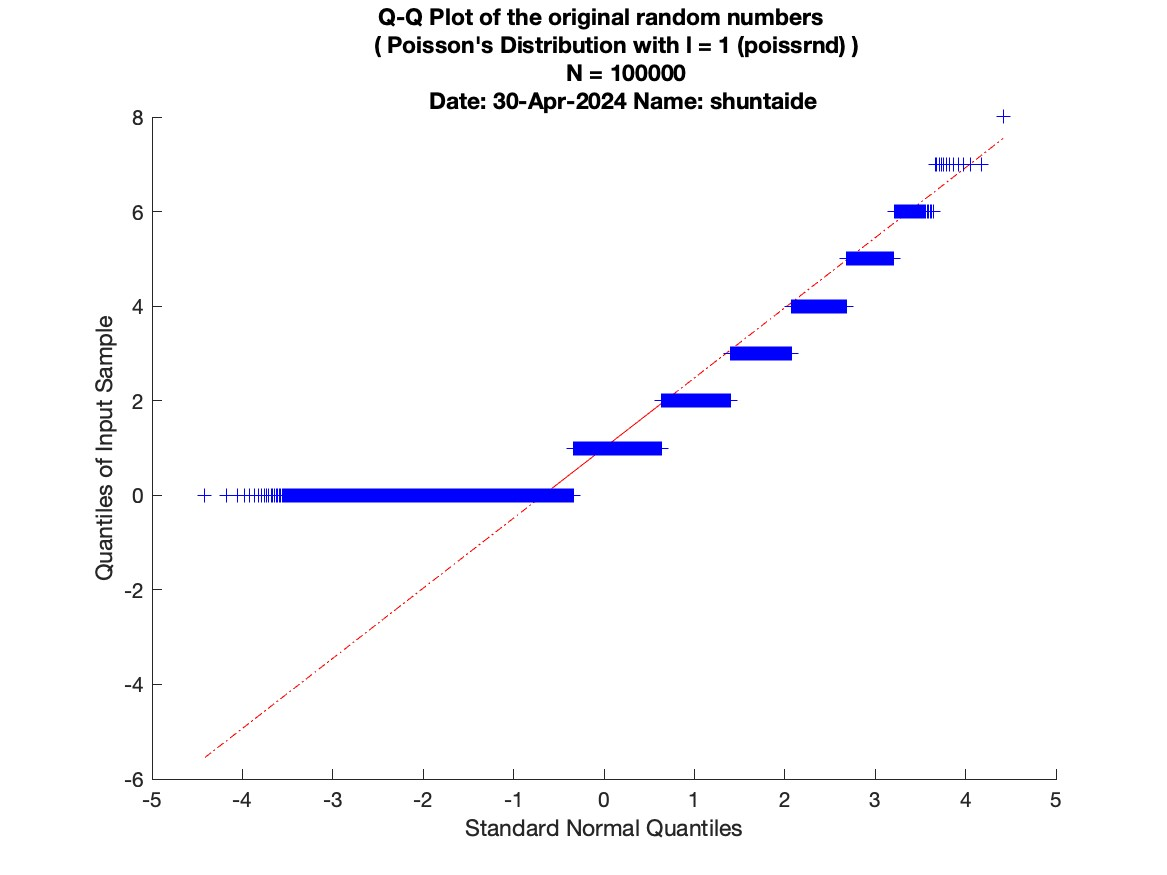
\includegraphics[width=0.8\textwidth]{src/figures/cl-poisson/cl_original_poissrnd_qqpl_N=100000.jpg}
		\subcaption{QQプロット}\label{fig:cl-poisson-original-qqpl}
	\end{subfigure}
	\begin{subfigure}{0.48\linewidth}
		\centering
		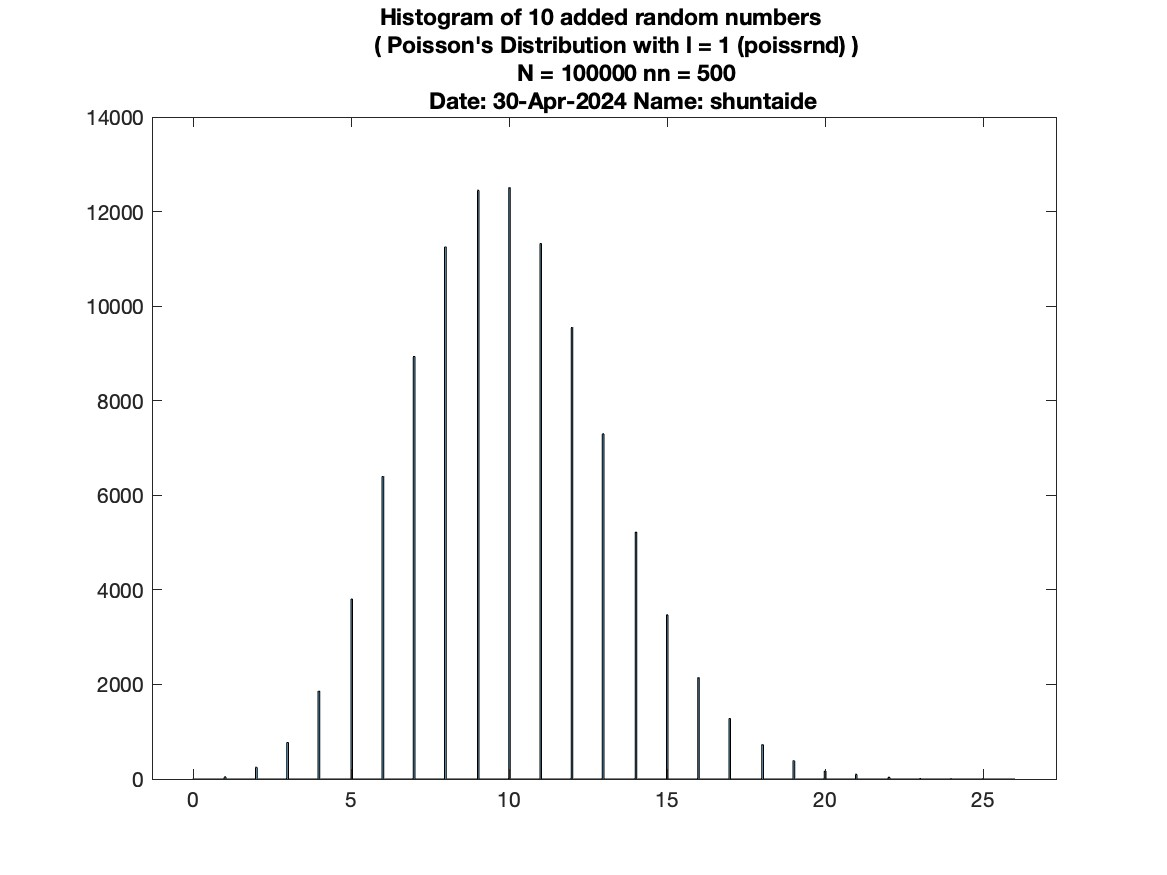
\includegraphics[width=0.8\textwidth]{src/figures/cl-poisson/cl_added_poissrnd_hist_N=100000_nn=500.jpg}
		\subcaption{加算後の分布}\label{fig:cl-poisson-added}
	\end{subfigure}
	\begin{subfigure}{0.48\linewidth}
		\centering
		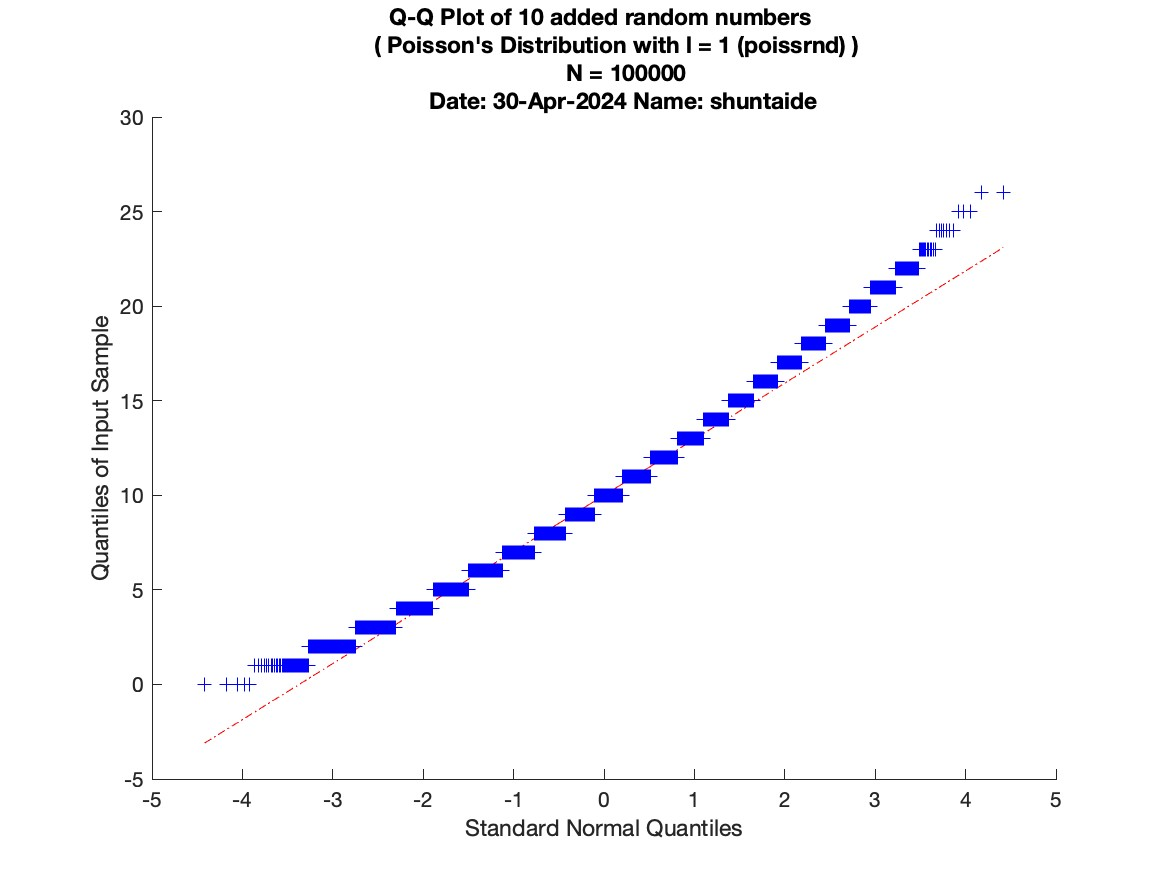
\includegraphics[width=0.8\textwidth]{src/figures/cl-poisson/cl_added_poissrnd_qqpl_N=100000.jpg}
		\subcaption{加算後のQQプロット}\label{fig:cl-poisson-added-qqpl}
	\end{subfigure}
	\caption{ポアソン分布による生成結果}\label{fig:cl-poisson-random}
\end{figure}

